% hack.
\gdef\currentsectionname{MailServers}
This section documents the most common mail (SMTP) and IMAPs/POPs servers. Another option to secure IMAPs/POPs servers is to place them behind an stunnel server.


%% ----------------------------------------------------------------------
\subsection{SMTP in general}
\label{subsection:smtp_general}
SMTP usually makes use of opportunistic TLS. This means that an MTA will accept TLS connections when asked for it during handshake but will not require it. One should always support incoming opportunistic TLS and always try TLS handshake outgoing.

Furthermore a mailserver can operate in three modes:
\begin{itemize*}
  \item As MSA (Mail Submission Agent) your mailserver receives mail from your clients MUAs (Mail User Agent).
  \item As receiving MTA (Mail Transmission Agent, MX)
  \item As sending MTA (SMTP client)
\end{itemize*}
We recommend the following basic setup for all modes:
\begin{itemize*}
  \item correctly setup MX, A and PTR RRs without using CNAMEs at all.
  \item enable encryption (opportunistic TLS)
  \item do not use self signed certificates
\end{itemize*}

For SMTP client mode we additionally recommend:
\begin{itemize*}
  \item the hostname used as HELO must match the PTR RR
  \item setup a client certificate (most server certificates are client certificates as well)
  \item either the common name or at least an alternate subject name of your certificate must match the PTR RR
  \item do not modify the cipher suite for client mode
\end{itemize*}

For MSA operation we recommend:
\begin{itemize*}
  \item listen on submission port 587
  \item enforce SMTP AUTH even for local networks
  \item do not allow SMTP AUTH on unencrypted connections
  \item optionally use the recommended cipher suites if (and only if) all your connecting MUAs support them
\end{itemize*}


% Note that (with the exception of MSA mode), it might be better to allow any cipher suite -- since any encryption is better than no encryption when it comes to opportunistic TLS.

We strongly recommend to allow all cipher suites for anything but MSA
mode, because the alternative is plain text transmission.

%% ----------------------------------------------------------------------
\subsection{Dovecot}


\subsubsection{Tested with Version}
\begin{itemize*}
  \item Dovecot 2.1.7, Debian Wheezy (without ``ssl\_prefer\_server\_ciphers'' setting)
  \item Dovecot 2.2.9, Debian Jessie
  \item 2.0.19apple1 on OS X Server 10.8.5 (without ``ssl\_prefer\_server\_ciphers'' setting)
  \item Dovecot 2.2.9 on Ubuntu 14.04 trusty
\end{itemize*}

\subsubsection{Settings}
% Example: http://dovecot.org/list/dovecot/2013-October/092999.html

\configfile{10-ssl.conf}{48-55}{Dovecot SSL configuration}

\subsubsection{Additional info}
Dovecot 2.0, 2.1: Almost as good as dovecot 2.2. Dovecot does not ignore unknown configuration parameters. Does not support
ssl\_prefer\_server\_ciphers

\subsubsection{Limitations}
Dovecot currently does not support disabling TLS compression. Furthermore, DH
parameters greater than 1024bit are not supported. The most recent version
2.2.7 of Dovecot implements configurable DH parameter length
\footnote{\url{http://hg.dovecot.org/dovecot-2.2/rev/43ab5abeb8f0}}.

%\subsubsection{Justification for special settings (if needed)}

% in case you have the need for further justifications why you chose this and that setting or if the settings do not fit into the standard Variant A or Variant B schema, please document this here

\subsubsection{References}
\begin{itemize*}
  \item \url{http://wiki2.dovecot.org/SSL}
\end{itemize*}

% add any further references or best practice documents here

\subsubsection{How to test}
% describe here or point the admin to tools (can be a simple footnote or \ref{} to  the tools section) which help the admin to test his settings.
\begin{lstlisting}
openssl s_client -crlf -connect SERVER.TLD:993
\end{lstlisting}


%% ----------------------------------------------------------------------
\subsection{cyrus-imapd}
\subsubsection{Tested with Versions}
\begin{itemize*}
  \item 2.4.17
\end{itemize*}

\subsubsection{Settings}

To activate SSL/TLS configure your certificate with
\configfile{imapd.conf}{206-206,209-209}{Activating TLS in cyrus}

Do not forget to add necessary intermediate certificates to the .pem file.

Limiting the ciphers provided may force (especially older) clients to connect without encryption at all! Sticking to the defaults is recommended.

If you still want to force strong encryption use
\configfile{imapd.conf}{263-263}{TLS cipher selection in cyrus}

cyrus-imapd loads hardcoded 1024 bit DH parameters using get\_rfc2409\_prime\_1024() by default. If you want to load your own DH parameters add them PEM encoded to the certificate file given in tls\_cert\_file. Do not forget to re-add them after updating your certificate.

To prevent unencrypted connections on the STARTTLS ports you can set
\configfile{imapd.conf}{131-131}{Force encrypted connections in cyrus}
This way MUAs can only authenticate with plain text authentication schemes after issuing the STARTTLS command. Providing CRAM-MD5 or DIGEST-MD5 methods is not recommended.

To support POP3/IMAP on ports 110/143 with STARTTLS and POP3S/IMAPS on ports
995/993 check the SERVICES section in \texttt{cyrus.conf}
\configfile{cyrus.conf}{28-28,31-34,71-71}{STARTTLS for POP3/IMAP and POP3S/IMAPS in cyrus}


\subsubsection{Limitations}
cyrus-imapd currently (2.4.17, trunk) does not support elliptic curve cryptography. Hence, ECDHE will not work even if defined in your cipher list.

Currently there is no way to prefer server ciphers or to disable compression.

There is a working patch for all three features:
\url{https://bugzilla.cyrusimap.org/show_bug.cgi?id=3823}

\subsubsection{How to test}
\begin{lstlisting}
openssl s_client -crlf -connect SERVER.TLD:993
\end{lstlisting}

% XXX config von Adi?
% sslVersion = TLSv1
% ciphers = EDH+CAMELLIA256:EDH+aRSA:+SSLv3:!aNULL:!eNULL:!LOW:!3DES:!MD5:!EXP:!PSK:!SRP:!DSS:!RC4:!SEED:-AES128:!CAMELLIA128:!ECDSA:AES256-SHA:EDH+AES128;
% options = CIPHER_SERVER_PREFERENCE
% TIMEOUTclose = 1


%% ----------------------------------------------------------------------
\subsection{Postfix}

\subsubsection{Tested with Versions}
\begin{itemize*}
  \item Postfix 2.9.6, Debian Wheezy with OpenSSL 1.0.1e
  \item Postfix 2.11.0 on Ubuntu 14.04.02 with OpenSSL 1.0.1f
\end{itemize*}


\subsubsection{Settings}

Postfix has five internal lists of ciphers, and the possibility to switch
between those with \emph{smtpd\_tls\_ciphers}. However, we leave this at its
default value for server to server connections, as many mail servers only
support outdated protocols and ciphers. We consider bad encryption still better
than plain text transmission. For connections to MUAs, TLS is mandatory and the
ciphersuite is modified.

%% I (cm) consider the generation of own DH parameters to be voodoo until
%% someone can explain the contrary. They are, after all, public, and
%% I found no research that would show that long-term use of a
%% parameter set would weaken the DH exchange. Also notice that IPSEC
%% uses fixed parameter sets only.
%&
%% also notice the following comment from  src/tls/tls_dh.c:
%% * Compiled-in EDH primes (the compiled-in generator is always 2). These are
%% * used when no parameters are explicitly loaded from a site-specific file.
%% *
%% * 512-bit parameters are used for export ciphers, and 1024-bit parameters are
%% * used for non-export ciphers. An ~80-bit strong EDH key exchange is really
%% * too weak to protect 128+ bit keys, but larger DH primes are
%% * computationally expensive. When greater security is required, use EECDH.

%% First, you need to generate Diffie Hellman parameters (please first take a look at the section \ref{section:RNGs}):

%% \todo{FIXME: this is a really weak setting! See also: http://postfix.1071664.n5.nabble.com/postfix-hardening-what-can-we-do-td61874.html}
%% \begin{lstlisting}
%%   % openssl gendh -out /etc/postfix/dh_param_512.pem -2 512
%%   % openssl gendh -out /etc/postfix/dh_param_1024.pem -2 1024
%% \end{lstlisting}

%% Next, we specify these DH parameters in \verb|main.cf|:

%% \begin{lstlisting}
%%   smtpd_tls_dh512_param_file = /etc/postfix/dh_param_512.pem
%%   smtpd_tls_dh1024_param_file = /etc/postfix/dh_param_1024.pem
%% \end{lstlisting}

\paragraph{MX and SMTP client configuration:}
As discussed in section \ref{subsection:smtp_general}, because of opportunistic
encryption we do not restrict the list of ciphers or protocols for communication
with other mail servers to avoid transmission in plain text. There are still
some steps needed to enable TLS, all in \verb|main.cf|:

\configfile{main.cf}{22-33}{Opportunistic TLS in Postfix}

\paragraph{MSA:}
For the MSA \verb|smtpd| process which communicates with mail clients, we first
define the ciphers that are acceptable for the ``mandatory'' security level,
again in \verb|main.cf|:

\configfile{main.cf}{35-37}{MSA TLS configuration in Postfix}

Then, we configure the MSA smtpd in \verb|master.cf| with two
additional options that are only used for this instance of smtpd:

\configfile{master.cf}{12-14}{MSA smtpd service configuration in Postfix}

For those users who want to use EECDH key exchange, it is possible to customize this via:
\configfile{main.cf}{38-38}{EECDH customization in Postfix}
The default value since Postfix 2.8 is ``strong''.

\subsubsection{Limitations}
tls\_ssl\_options is supported from Postfix 2.11 onwards. You can
leave the statement in the configuration for older versions, it will
be ignored.

tls\_preempt\_cipherlist is supported from Postfix 2.8 onwards. Again,
you can leave the statement in for older versions.

\subsubsection{References}
Refer to \url{http://www.postfix.org/TLS_README.html} for an in-depth
discussion.

\subsubsection{Additional settings}
Postfix has two sets of built-in DH parameters that can be overridden
with the \verb|smtpd_tls_dh512_param_file|
and \verb|smtpd_tls_dh1024_param_file| options. The ``dh512''
parameters are used for export ciphers, while the ``dh1024'' ones are
used for all other ciphers.

The ``bit length'' in those parameter names is just a name, so one
could use stronger parameter sets; it should be possible to e.g. use the
IKE Group14 parameters (see section \ref{section:DH}) without much
interoperability risk, but we have not tested this yet.

% \subsubsection{Justification for special settings (if needed)}
% no special settings


\subsubsection{How to test}
You can check the effect of the settings with the following command:
\begin{lstlisting}
$ zegrep "TLS connection established from.*with cipher" /var/log/mail.log | awk '{printf("%s %s %s %s\n", $12, $13, $14, $15)}' | sort | uniq -c | sort -n
      1 SSLv3 with cipher DHE-RSA-AES256-SHA
     23 TLSv1.2 with cipher DHE-RSA-AES256-GCM-SHA384
     60 TLSv1 with cipher ECDHE-RSA-AES256-SHA
    270 TLSv1.2 with cipher ECDHE-RSA-AES256-GCM-SHA384
    335 TLSv1 with cipher DHE-RSA-AES256-SHA
\end{lstlisting}

\begin{lstlisting}
openssl s_client -starttls smtp -crlf -connect SERVER.TLD:25
\end{lstlisting}

%% ----------------------------------------------------------------------

\subsection{Exim}

\subsubsection{Tested with Versions}
\begin{itemize*}
  \item Exim 4.82, Debian Jessie
  \item Exim 4.82, Ubuntu 14.04.2 with OpenSSL 1.0.1e
\end{itemize*}


It is highly recommended to read
\url{http://exim.org/exim-html-current/doc/html/spec_html/ch-encrypted_smtp_connections_using_tlsssl.html}
first.

\paragraph{MSA mode (submission):}
In the main config section of Exim add:
\configfile{configure.msa}{153-154}{Certificate selection in Exim (MSA)}
Don't forget to add intermediate certificates to the .pem file if needed.

Tell Exim to advertise STARTTLS in the EHLO answer to everyone:
\configfile{configure.msa}{145-145}{TLS advertise in Exim (MSA)}

If you want to support legacy SMTPS on port 465, and STARTTLS on smtp(25)/submission(587) ports set
\configfile{configure.msa}{165-166}{STARTTLS and SMTPS in Exim (MSA)}

It is highly recommended to limit SMTP AUTH to SSL connections only. To do so add
\configfile{configure.msa}{813-813}{SSL-only authentication in Exim (MSA)}
to every authenticator defined.

Add the following rules on top of your acl\_smtp\_mail:
\configfile{configure.msa}{111-111,501-505}{Submission mode in Exim (MSA)}
This switches Exim to submission mode and allows addition of missing ``Message-ID'' and ``Date'' headers.

It is not advisable to restrict the default cipher list for MSA mode if you don't know all connecting MUAs. If you still want to define one please consult the Exim documentation or ask on the exim-users mailinglist.
% Exim maintainers do not recommend to change default ciphers
% I think we shouldn't, too
%use:
%\begin{lstlisting}
%  tls_require_ciphers = <...recommended ciphersuite...>
%\end{lstlisting}

The cipher used is written to the logfiles by default. You may want to add
\begin{lstlisting}
log_selector = <whatever your log_selector already contains> +tls_certificate_verified +tls_peerdn +tls_sni
\end{lstlisting}
to get even more TLS information logged.


\paragraph{Server mode (incoming):}
In the main config section of Exim add:
\configfile{configure.server}{152-153}{Certificate selection in Exim (Server)}
don't forget to add intermediate certificates to the .pem file if needed.

Tell Exim to advertise STARTTLS in the EHLO answer to everyone:
\configfile{configure.server}{144-144}{TLS advertise in Exim (Server)}

Listen on smtp(25) port only
\configfile{configure.server}{166-166}{STARTTLS on SMTP in Exim (Server)}

It is not advisable to restrict the default cipher list for opportunistic encryption as used by SMTP. Do not use cipher lists recommended for HTTPS! If you still want to define one please consult the Exim documentation or ask on the exim-users mailinglist.
% Exim maintainers do not recommend to change default ciphers
% We shouldn't, too
%use:
%\begin{lstlisting}
%  tls_require_ciphers = <...recommended ciphersuite...>
%\end{lstlisting}

If you want to request and verify client certificates from sending hosts set
\configfile{configure.server}{154-155}{TLS certificate verifiaction in Exim (Server)}

tls\_try\_verify\_hosts only reports the result to your logfile. If you want to disconnect such clients you have to use
\begin{lstlisting}
tls_verify_hosts = *
\end{lstlisting}

The cipher used is written to the logfiles by default. You may want to add
\begin{lstlisting}
log_selector = <whatever your log_selector already contains> +tls_certificate_verified +tls_peerdn +tls_sni
\end{lstlisting}
to get even more TLS information logged.

\paragraph{Client mode (outgoing):}
Exim uses opportunistic encryption in the SMTP transport by default.

Client mode settings have to be done in the configuration section of the smtp transport (driver = smtp).

If you want to use a client certificate (most server certificates can be used as client certificate, too) set
\configfile{configure.client}{152-153}{Certificate selection in Exim (Client)}
This is recommended for MTA-MTA traffic.

%If you want to limit used ciphers set
%\begin{lstlisting}
%  tls_require_ciphers = <...recommended ciphersuite...>
%\end{lstlisting}
% Exim Maintainers do not recommend ciphers. We shouldn't do so, too.
Do not limit ciphers without a very good reason. In the worst case you end up without encryption at all instead of some weak encryption. Please consult the Exim documentation if you really need to define ciphers.

\paragraph{OpenSSL:}
Exim already disables SSLv2 by default. We recommend to add
\begin{lstlisting}
openssl_options = +all +no_sslv2 +no_compression +cipher_server_preference
\end{lstlisting}
to the main configuration.

Note: +all is misleading here since OpenSSL only activates the most common workarounds. But that's how SSL\_OP\_ALL is defined.

You do not need to set dh\_parameters. Exim with OpenSSL by default uses parameter initialization with the "2048-bit MODP Group with 224-bit Prime Order Subgroup" defined in section 2.2 of RFC 5114~\cite{rfc5114} (ike23).
If you want to set your own DH parameters please read the TLS documentation of exim.


\paragraph{GnuTLS:}
GnuTLS is different in only some respects to OpenSSL:
\begin{itemize*}
  \item tls\_require\_ciphers needs a GnuTLS priority string instead of a cipher list. It is recommended to use the defaults by not defining this option. It highly depends on the version of GnuTLS used. Therefore it is not advisable to change the defaults.
  \item There is no option like openssl\_options
\end{itemize*}

\paragraph{Exim string expansion:}
Note that most of the options accept expansion strings. This way you can e.g. set cipher lists or STARTTLS advertisement conditionally. Please follow the link to the official Exim documentation to get more information.

\paragraph{Limitations:}
Exim currently (4.82) does not support elliptic curves with OpenSSL. This means that ECDHE is not used even if defined in your cipher list.
There already is a working patch to provide support:
\url{http://bugs.exim.org/show_bug.cgi?id=1397}

\subsubsection{How to test}
\begin{lstlisting}
openssl s_client -starttls smtp -crlf -connect SERVER.TLD:25
\end{lstlisting}


%% ----------------------------------------------------------------------
%\subsection{Exchange}

%\todo{FIXME: write this section}

%% ----------------------------------------------------------------------
\subsection{Cicso ESA/IronPort}
\subsubsection{Tested with Version}
\begin{itemize*}
  \item AsyncOS 7.6.1
  \item AsyncOS 8.5.6
  \item AsyncOS 9.0.0 and 9.1.0
\end{itemize*}

\subsubsection{Settings}
Import your certificate(s) using the WEBUI (Network -> Certificates).

From AsyncOS 9.0 and up, SSL parameters for inbound SMTP, outbound SMTP and GUI access can be configured in one step via the WEBUI (System Administration -> SSL Configuration, see figure \ref{fig:ach_ironport_ssl_settings} on page \pageref{fig:ach_ironport_ssl_settings}). \\
For all versions prior to 9.0, you have to connect to the CLI and configure the SSL parameters separately, as shown below using inbound SMTP as example.
\begin{lstlisting}{foo}
ironport.example.com> sslconfig
sslconfig settings:
  GUI HTTPS method:  sslv3tlsv1
  GUI HTTPS ciphers: RC4-SHA:RC4-MD5:ALL
  Inbound SMTP method:  sslv3tlsv1
  Inbound SMTP ciphers: RC4-SHA:RC4-MD5:ALL
  Outbound SMTP method:  sslv3tlsv1
  Outbound SMTP ciphers: RC4-SHA:RC4-MD5:ALL
	
Choose the operation you want to perform:
- GUI - Edit GUI HTTPS ssl settings.
- INBOUND - Edit Inbound SMTP ssl settings.
- OUTBOUND - Edit Outbound SMTP ssl settings.
- VERIFY - Verify and show ssl cipher list.
[]> inbound

Enter the inbound SMTP ssl method you want to use.
1. SSL v2.
2. SSL v3
3. TLS v1
4. SSL v2 and v3
5. SSL v3 and TLS v1
6. SSL v2, v3 and TLS v1
[5]> 3

Enter the inbound SMTP ssl cipher you want to use.
[RC4-SHA:RC4-MD5:ALL]> EDH+CAMELLIA:EDH+aRSA:EECDH+aRSA+AESGCM:EECDH+aRSA+SHA256:EECDH:+CAMELLIA128:+AES128:+SSLv3:!aNULL:!eNULL:!LOW:!3DES:!MD5:!EXP:!PSK:!DSS:!RC4:!SEED:!IDEA:!ECDSA:kEDH:CAMELLIA128-SHA:AES128-SHA

sslconfig settings:
  GUI HTTPS method:  sslv3tlsv1
  GUI HTTPS ciphers: RC4-SHA:RC4-MD5:ALL
  Inbound SMTP method:  tlsv1
  Inbound SMTP ciphers: EDH+CAMELLIA:EDH+aRSA:EECDH+aRSA+AESGCM:EECDH+aRSA+SHA384:EECDH+aRSA+SHA256:EECDH:+CAMELLIA256:+AES256:+CAMELLIA128:+AES128:+SSLv3:!aNULL:!eNULL:!LOW:!3DES:!MD5:!EXP:!PSK:!SRP:!DSS:!RC4:!SEED:!ECDSA:CAMELLIA256-SHA:AES256-SHA:CAMELLIA128-SHA:AES128-SHA
  Outbound SMTP method:  sslv3tlsv1
  Outbound SMTP ciphers: RC4-SHA:RC4-MD5:ALL
\end{lstlisting}
Note that starting with AsyncOS 9.0 SSLv3 is disabled by default, whereas the default cipher set is still \texttt{RC4-SHA:RC4-MD5:ALL} (see figure \ref{fig:ach_ironport_ssl_settings} on page \pageref{fig:ach_ironport_ssl_settings}). 

\begin{figure}[p]
  \centering
  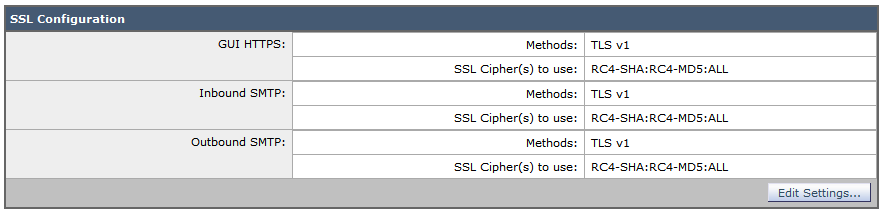
\includegraphics[width=0.8\textwidth]{img/ach_ironport_ssl_settings.png}
  \caption{Default SSL Settings}
  \label{fig:ach_ironport_ssl_settings}
\end{figure}

After committing these changes in the CLI, you have to activate the use of TLS in several locations. 

For inbound connections, first select the appropriate certificate in the settings of each listener you want to have TLS enabled on (Network -> Listeners, see figure \ref{fig:ach_ironport_listener_cert} on page \pageref{fig:ach_ironport_listener_cert}). Afterwards, for each listener, configure all Mail Flow Policies which have their Connection Behavior set to ``Accept'' or ``Relay'' to at least prefer TLS (Mail Policies -> Mail Flow Policies, see figure \ref{fig:ach_ironport_mail_flow_tls} on page \pageref{fig:ach_ironport_mail_flow_tls}). \\
It is recommended to also enable TLS in the default Mail Flow Policy, because these settings will be inherited by newly created policies, unless specifically overwritten. \\
TLS can be enforced by creating a new Mail Flow Policy with TLS set to ``required'', creating a new Sender Group defining the addresses of the sending mail servers for which you want to enforce encryption (Mail Policies -> HAT Overview) and using this new Sender Group in conjunction with the newly created Mail Flow Policy. 

\begin{figure}[p]
  \centering
  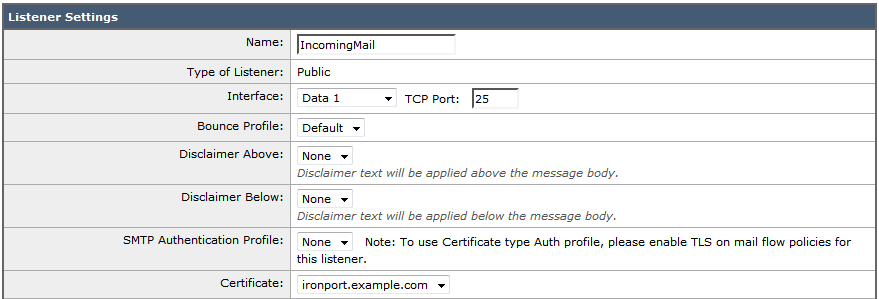
\includegraphics[width=0.8\textwidth]{img/ach_ironport_listener_cert.png}
  \caption{Listener Settings}
  \label{fig:ach_ironport_listener_cert}
\end{figure}

\begin{figure}[p]
  \centering
  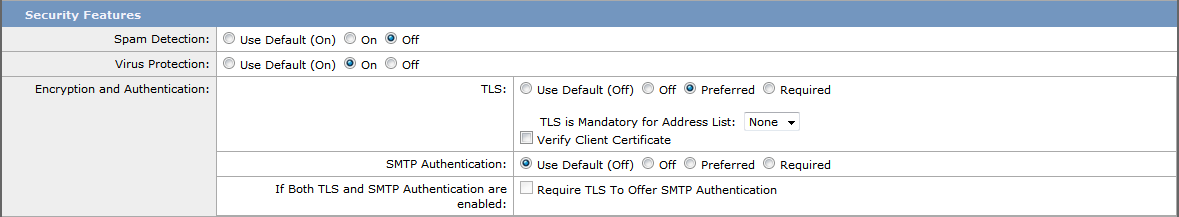
\includegraphics[width=0.8\textwidth]{img/ach_ironport_mail_flow_tls.png}
  \caption{Mail Flow Policy Security Features}
  \label{fig:ach_ironport_mail_flow_tls}
\end{figure}

TLS settings for outbound connections have to be configured within the Destination Controls (Mail Policies -> Destination Controls). Chose the appropriate SSL certificate within the global settings and configure TLS to be preferred in the default profile to enable it for all outbound connections. After these two steps the Destination Control overview page should look like figure \ref{fig:ach_ironport_dest_control} on page \pageref{fig:ach_ironport_dest_control}. 
To enforce TLS for a specific destination domain, add an entry to the Destination Control Table and set ``TLS Support'' to ``required''.

\begin{figure}[p]
  \centering
  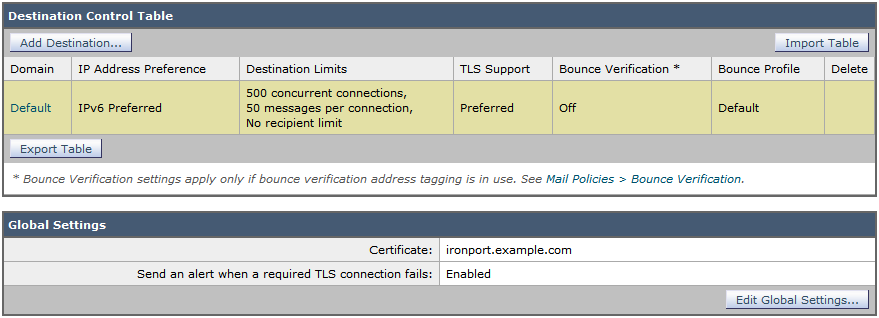
\includegraphics[width=0.8\textwidth]{img/ach_ironport_dest_control.png}
  \caption{Destination Control overview}
  \label{fig:ach_ironport_dest_control}
\end{figure}

\subsubsection{Limitations}
All current AsyncOS versions use OpenSSL 0.9.8. Therefore TLS 1.2 is not supported and some of the suggested ciphers won't work. According to Cisco, implementation of TLS 1.2 is on the road map for AsyncOS 9.5.\footnote{\url{https://twitter.com/CiscoEmailSec/status/562974300379308033}} You can check the supported ciphers on the CLI by using the option \texttt{verify} from within the \texttt{sslconfig} command:
\begin{lstlisting}{foo}
[]> verify

Enter the ssl cipher you want to verify.
[]> EDH+CAMELLIA:EDH+aRSA:EECDH+aRSA+AESGCM:EECDH+aRSA+SHA256:EECDH:+CAMELLIA128:+AES128:+SSLv3:!aNULL:!eNULL:!LOW:!3DES:!MD5:!EXP:!PSK:!DSS:!RC4:!SEED:!IDEA:!ECDSA:kEDH:CAMELLIA128-SHA:AES128-SHA

DHE-RSA-CAMELLIA256-SHA SSLv3 Kx=DH       Au=RSA  Enc=Camellia(256) Mac=SHA1
DHE-RSA-CAMELLIA128-SHA SSLv3 Kx=DH       Au=RSA  Enc=Camellia(128) Mac=SHA1
DHE-RSA-AES256-SHA      SSLv3 Kx=DH       Au=RSA  Enc=AES(256)  Mac=SHA1
DHE-RSA-AES128-SHA      SSLv3 Kx=DH       Au=RSA  Enc=AES(128)  Mac=SHA1
CAMELLIA128-SHA         SSLv3 Kx=RSA      Au=RSA  Enc=Camellia(128) Mac=SHA1
AES128-SHA              SSLv3 Kx=RSA      Au=RSA  Enc=AES(128)  Mac=SHA1
\end{lstlisting}

\subsubsection{How to test}
\begin{lstlisting}
openssl s_client -starttls smtp -crlf -connect SERVER.TLD:25
\end{lstlisting}

\FloatBarrier % the preceding section has several figures. Floating them too far away might get confusing for readers.